\documentclass[10pt,a4paper]{article}
\usepackage[margin=21mm,headheight=14pt]{geometry}
\usepackage[T1]{fontenc}
\usepackage{lmodern,microtype,amsmath,amssymb,bm,booktabs,array,graphicx}
\usepackage{siunitx,xcolor,enumitem,fancyhdr,caption,float}
\usepackage{tikz}
\usetikzlibrary{arrows.meta,calc,decorations.markings}
\usepackage[hyphens]{url}
\usepackage{xurl}
\usepackage[colorlinks=true,linkcolor=blue!45!black,urlcolor=blue!45!black]{hyperref}
\usepackage[nameinlink,noabbrev]{cleveref}
\hypersetup{pdftitle={Uniform IPPL grid and curved-source field operator},pdfauthor={OPALX numerical validation},pdfsubject={Mapped coordinates and nonlocal FFT2D5 OPEN implementation}}
\setlength{\parindent}{0pt}
\setlength{\parskip}{5pt plus 1pt}
\setlist{nosep,leftmargin=1.5em}
\captionsetup{font=small,labelfont=bf}
\pagestyle{fancy}\fancyhf{}
\fancyhead[L]{\small OPALX / mapped-grid field operator}
\fancyhead[R]{\small Technical note / 3 November 2026}
\fancyfoot[C]{\thepage}
\newcommand{\dd}{\mathrm d}
\newcommand{\eps}{\epsilon_0}
\newcommand{\code}[1]{{\small\nolinkurl{#1}}}
\begin{document}
\section{Uniform IPPL grid and curved-source field operator}
\label{sec:mapped-grid}

\subsection{What the grid represents}
IPPL still stores a uniform Cartesian grid. No curved-mesh class, curved-cell
connectivity or general curvilinear Poisson solver has been added to IPPL.
The new OPALX OPEN backend interprets the three array coordinates as radial
offset $u$, vertical offset $y$ and reference-path arc length $s$. OPALX supplies
the coordinate map, the curvature-dependent Coulomb operator and the field
transformations. IPPL supplies uniform field storage and FFT operations.

\begin{figure}[H]
 \centering
 % Mapped-grid schematic, not an IPPL curved-mesh implementation.
% Physical centreline: X=((R+u)cos(s/R)-R,y,(R+u)sin(s/R)); R=2 m.
% The origin of s is shifted to the charged-beam midpoint for this figure.
% Visible physical tube thickness and grid spacing are deliberately schematic.
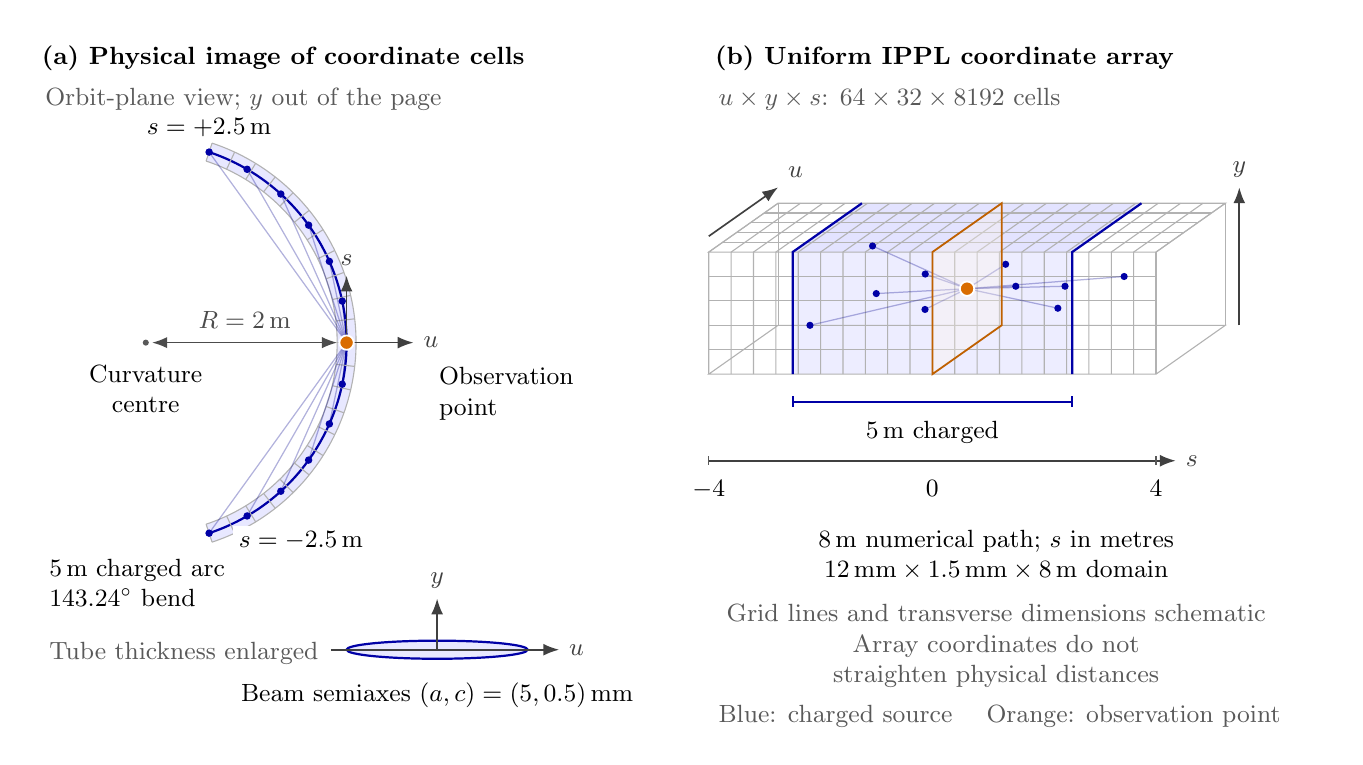
\begin{tikzpicture}[
  x=1cm,y=1cm,font=\small,>=Latex,
  mggrid/.style={line width=.4pt,black!30},
  mgsource/.style={blue!65!black,line width=.8pt},
  mgcoupling/.style={blue!55!black,opacity=.3,line width=.45pt},
  mgaxis/.style={->,black!75,line width=.6pt},
  mgdim/.style={<->,black!70,line width=.55pt},
  mgtarget/.style={fill=orange!85!black,draw=white,line width=.65pt},
  mglabel/.style={fill=white,inner sep=2pt}
]
 \path[use as bounding box] (0,0) rectangle (16.6,9.0);
 \node[anchor=north west,font=\bfseries\small,align=left,text width=7.4cm]
   at (.1,8.9) {(a) Physical image of coordinate cells};
 \node[anchor=north west,font=\bfseries\small,align=left,text width=7.7cm]
   at (8.65,8.9) {(b) Uniform IPPL coordinate array};
 \node[anchor=north west,black!65] at (.1,8.35)
   {Orbit-plane view; $y$ out of the page};
 \node[anchor=north west,black!65] at (8.65,8.35)
   {$u\times y\times s$: $64\times32\times8192$ cells};

 % Physical circular arc: theta=s/R, -1.25 <= theta <= 1.25 rad.
 \coordinate (mgO) at (1.5,5.0);
 \coordinate (mgT) at ($(mgO)+(0:2.55)$);
 \fill[blue!9] ($(mgO)+(-71.619724:2.43)$)
   arc[start angle=-71.619724,end angle=71.619724,radius=2.43]
   -- ($(mgO)+(71.619724:2.67)$)
   arc[start angle=71.619724,end angle=-71.619724,radius=2.67] -- cycle;
 \foreach \rad in {2.43,2.67} {
   \draw[mggrid] ($(mgO)+(-71.619724:\rad)$)
     arc[start angle=-71.619724,end angle=71.619724,radius=\rad];
 }
 \draw[mgsource] ($(mgO)+(-71.619724:2.55)$)
   arc[start angle=-71.619724,end angle=71.619724,radius=2.55];
 \foreach \theta in {-71.619724,-65,-58.5,-52,-45.5,-39,-32.5,-26,-19.5,-13,-6.5,0,6.5,13,19.5,26,32.5,39,45.5,52,58.5,65,71.619724} {
   \draw[mggrid] ($(mgO)+(\theta:2.43)$) -- ($(mgO)+(\theta:2.67)$);
 }
 \foreach \theta in {-71.619724,-59.6831,-47.7465,-35.8099,-23.8732,-11.9366,11.9366,23.8732,35.8099,47.7465,59.6831,71.619724} {
   \draw[mgcoupling] ($(mgO)+(\theta:2.55)$) -- (mgT);
   \fill[blue!65!black] ($(mgO)+(\theta:2.55)$) circle[radius=1.35pt];
 }
 \fill[black!65] (mgO) circle[radius=1.1pt];
 \draw[mgdim] ($(mgO)+(.08,0)$) -- ($(mgT)+(-.12,0)$)
   node[midway,above=3pt,mglabel] {$R=2\,\mathrm m$};
 \node[anchor=north,align=center] at ($(mgO)+(0,-.16)$)
   {Curvature\\centre};
 \draw[mgaxis] (mgT) -- ($(mgT)+(.85,0)$) node[right] {$u$};
 \draw[mgaxis] (mgT) -- ($(mgT)+(0,.85)$) node[above] {$s$};
 \fill[mgtarget] (mgT) circle[radius=2.6pt];
 \node[anchor=west,align=left] at ($(mgT)+(1.05,-.65)$)
   {Observation\\point};
 \node[anchor=south,mglabel] at ($(mgO)+(71.619724:2.55)+(0,.12)$)
   {$s=+2.5\,\mathrm m$};
 \node[anchor=west,mglabel] at ($(mgO)+(-71.619724:2.55)+(.3,-.1)$)
   {$s=-2.5\,\mathrm m$};
 \node[anchor=west,align=left] at (.15,1.95)
   {$5\,\mathrm m$ charged arc\\$143.24^\circ$ bend};
 \node[anchor=west,black!65] at (.15,1.05)
   {Tube thickness enlarged};

 % True transverse aspect ratio a/c=10, drawn at a separate magnification.
 \coordinate (mgS) at (5.2,1.1);
 \draw[mgsource,fill=blue!9] (mgS) ellipse[x radius=1.15,y radius=.115];
 \draw[mgaxis] ($(mgS)+(-1.35,0)$) -- ($(mgS)+(1.55,0)$) node[right] {$u$};
 \draw[mgaxis] (mgS) -- ($(mgS)+(0,.65)$) node[above] {$y$};
 \node[anchor=north,align=center] at ($(mgS)+(0,-.3)$)
   {Beam semiaxes $(a,c)=(5,0.5)\,\mathrm{mm}$};

 % A rectangular array in logical coordinates. s is long; u is the slanted
 % depth direction; y is vertical. Physical aspect ratios are not drawn to scale.
 \begin{scope}[shift={(8.65,4.6)},x={(.71cm,0cm)},y={(.88cm,.62cm)},z={(0cm,1.55cm)}]
   \fill[blue!11] (1.5,0,1) -- (6.5,0,1) -- (6.5,1,1) -- (1.5,1,1) -- cycle;
   \fill[blue!7] (1.5,0,0) -- (6.5,0,0) -- (6.5,0,1) -- (1.5,0,1) -- cycle;
   \draw[mggrid] (0,0,0) -- (8,0,0) -- (8,1,0) -- (0,1,0) -- cycle;
   \draw[mggrid] (0,0,1) -- (8,0,1) -- (8,1,1) -- (0,1,1) -- cycle;
   \foreach \ss in {0,8} {
     \foreach \uu in {0,1} {\draw[mggrid] (\ss,\uu,0) -- (\ss,\uu,1);}
   }
   \foreach \ss in {0,.4,...,8} {
     \draw[mggrid] (\ss,0,0) -- (\ss,0,1) -- (\ss,1,1);
   }
   \foreach \qq in {.2,.4,.6,.8} {
     \draw[mggrid] (0,0,\qq) -- (8,0,\qq);
     \draw[mggrid] (0,\qq,1) -- (8,\qq,1);
   }
   \foreach \ss in {1.5,6.5} {
     \draw[mgsource] (\ss,0,0) -- (\ss,0,1) -- (\ss,1,1);
   }
   \foreach \ss/\uu/\yy in {1.5/.25/.3,2/.75/.75,2.5/.4/.5,3/.7/.25,3.5/.3/.7,4.5/.8/.4,5/.25/.8,5.5/.6/.3,6/.3/.6,6.5/.75/.5} {
     \draw[mgcoupling] (\ss,\uu,\yy) -- (4,.5,.5);
     \fill[blue!65!black] (\ss,\uu,\yy) circle[radius=1.3pt];
   }
   \draw[orange!75!black,line width=.65pt,fill=orange!7,fill opacity=.35]
     (4,0,0) -- (4,0,1) -- (4,1,1) -- (4,1,0) -- cycle;
   \fill[mgtarget] (4,.5,.5) circle[radius=2.6pt];
   \draw[mgaxis] (0,0,1.13) -- (0,1,1.13) node[above right] {$u$};
   \draw[mgaxis] (8.25,1,0) -- (8.25,1,1.13) node[above] {$y$};
   \coordinate (mgAL) at (0,0,0);
   \coordinate (mgAR) at (8,0,0);
   \coordinate (mgCL) at (1.5,0,0);
   \coordinate (mgCR) at (6.5,0,0);
 \end{scope}
 \draw[mgsource] ($(mgCL)+(0,-.35)$) -- ($(mgCR)+(0,-.35)$);
 \foreach \pp in {mgCL,mgCR} {\draw[mgsource] ($(\pp)+(0,-.28)$) -- ($(\pp)+(0,-.42)$);}
 \node[anchor=north] at ($(mgCL)!.5!(mgCR)+(0,-.48)$) {$5\,\mathrm m$ charged};
 \draw[mgaxis] ($(mgAL)+(0,-1.1)$) -- ($(mgAR)+(.25,-1.1)$) node[right] {$s$};
 \foreach \pp/\val in {mgAL/-4,mgAR/4} {
   \draw[black!65,line width=.5pt] ($(\pp)+(0,-1.04)$) -- ($(\pp)+(0,-1.16)$);
   \node[anchor=north] at ($(\pp)+(0,-1.23)$) {$\val$};
 }
 \node[anchor=north] at ($(mgAL)!.5!(mgAR)+(0,-1.23)$) {$0$};
 \node[align=center] at (12.3,2.3)
   {$8\,\mathrm m$ numerical path; $s$ in metres\\
    $12\,\mathrm{mm}\times1.5\,\mathrm{mm}\times8\,\mathrm m$ domain};
 \node[align=center,black!65,text width=7.5cm] at (12.3,1.15)
   {Grid lines and transverse dimensions schematic\\
    Array coordinates do not straighten physical distances};
 \node[anchor=west,black!65] at (8.65,.25)
   {Blue: charged source \quad Orange: observation point};
\end{tikzpicture}

 \caption{Two representations of the same source. Left: the physical image of
 reference-path coordinate cells on a circular arc, with transverse thickness
 enlarged. Right: the ordinary rectangular IPPL array indexed by $(u,y,s)$.
 The rectangular drawing does not straighten the source in the Coulomb
 calculation. Lines joining source sections to an observation point illustrate
 nonlocal coupling, not computed field vectors or magnitudes. Only a schematic
 subset of grid lines is drawn; the empty interior of the bend is not meshed.}
 \label{fig:mg-geometry}
\end{figure}

\begin{center}\small
\begin{tabular}{ll}\toprule
Quantity & Frozen-field benchmark\\\midrule
Charged length; bending radius & $L=5$ m; $R=2$ m\\
Total source angle; radial thinness & $L/R=2.5$ rad $=143.24^\circ$; $a/R=0.0025$\\
Radial / vertical source semiaxes & $a=5$ mm; $c=0.5$ mm\\
Uniform coordinate domain & $12$ mm $\times1.5$ mm $\times8$ m\\
Primary field grid & $64\times32\times8192$ cells\\\bottomrule
\end{tabular}
\end{center}

This is a nonlocal three-dimensional field calculation specialized to a thin
circular tube, selected through the existing \code{FFT2D5} interface. It
replaces the OPEN slice calculation; it is more than a correction to a local
longitudinal coefficient. The other pipe modes retain their separate slice
calculations and longitudinal closures.

\clearpage
\subsection{Coordinate map and charge deposition}
For an explanatory circle centred at $(-R,0,0)$, choose $s=0$ at the middle
of the charged arc and define
\begin{equation}
 \bm X(u,y,s)=
 \begin{pmatrix}(R+u)\cos(s/R)-R\\ y\\(R+u)\sin(s/R)\end{pmatrix},
 \qquad -L/2\le s\le L/2.
 \label{eq:mg-map}
\end{equation}
The implementation instead starts $s=0$ at the first reference-path point.
An arc-length origin shift and a rigid rotation/translation connect the two
conventions. They do not change source-target separations or the calculation.
Path and particle coordinates are placed in one common solve frame.

For $\kappa=1/R$, the local radial, vertical and tangent unit vectors are
\begin{equation}
 \bm e_u=(\cos\kappa s,0,\sin\kappa s),\quad
 \bm e_y=(0,1,0),\quad
 \bm e_s=(-\sin\kappa s,0,\cos\kappa s).
 \label{eq:mg-basis}
\end{equation}
The coordinate scale factors are $(1,1,h)$, where
\begin{equation}
 h(u)=1+\kappa u,\qquad
 \dd\ell^2=\dd u^2+\dd y^2+h^2\dd s^2,\qquad
 \dd V=h\,\dd u\,\dd y\,\dd s.
 \label{eq:mg-metric}
\end{equation}
Thus uniform intervals in $s$ are uniform reference-path arc intervals.
At a radial offset $u$, their physical tangential length is $h\,\Delta s$.
The mapped physical cells have different tangential lengths even though the
IPPL coordinate spacing is constant.

OPALX first maps each particle position to $(u,y,s)$ and then applies ordinary
cloud-in-cell deposition on that uniform coordinate grid. Its cell centres are
\begin{equation}
 (u_i,y_j,s_k)=
 (u_{\min}+(i+\tfrac12)\Delta u,\;
  y_{\min}+(j+\tfrac12)\Delta y,\;
  s_{\min}+(k+\tfrac12)\Delta s).
 \label{eq:mg-grid}
\end{equation}
The primary spacings are $\Delta u=0.1875$ mm, $\Delta y=0.046875$ mm and
$\Delta s=0.9765625$ mm. The stored source is charge per \emph{coordinate}
volume, not charge per physical volume:
\begin{equation}
 \rho_c=\frac{\dd q}{\dd u\,\dd y\,\dd s}
       =h\rho_{\rm phys},\qquad
 \int\rho_c\,\dd u\,\dd y\,\dd s=Q.
 \label{eq:mg-density}
\end{equation}
Depositing actual particle charges already represents this Jacobian. Applying
an additional factor $h$ to the deposited source would count it twice. A
uniform physical density therefore corresponds to coordinate density
proportional to $h$, rather than a constant array value.

Merely mapping coordinates and calling a Cartesian Poisson solver would omit
the geometric terms. For constant curvature, the physical Laplacian is
\begin{equation}
 \nabla^2\Phi=\frac1h\partial_u(h\partial_u\Phi)
       +\partial_y^2\Phi+\frac1{h^2}\partial_s^2\Phi.
 \label{eq:mg-laplacian}
\end{equation}
The current backend does not discretize this mapped PDE. It instead constructs
an approximate physical free-space Green function and evaluates its integral.

\clearpage
\subsection{How the curved Coulomb interaction becomes FFT convolutions}
In the low-speed curved case, the electrostatic potential is
\begin{equation}
 \Phi(u,y,s)=\frac1{4\pi\eps}
 \int\frac{\rho_c(u',y',s')}{d(u,y,s;u',y',s')}
           \,\dd u'\,\dd y'\,\dd s',
 \label{eq:mg-exact-potential}
\end{equation}
where $d=|\bm X(u,y,s)-\bm X(u',y',s')|$ is a physical Cartesian distance.
For a circular reference, introduce $x=u-u'$, $v=y-y'$ and $\tau=s-s'$.
The exact squared distance is
\begin{align}
 \xi(\tau)&=\frac{2\sin(\kappa\tau/2)}{\kappa},\qquad
 D^2=x^2+v^2+\xi^2,\nonumber\\
 d^2&=x^2+v^2+\xi^2(1+\kappa u)(1+\kappa u')
     =D^2+\xi^2[\kappa(u+u')+\kappa^2uu'].
 \label{eq:mg-distance}
\end{align}
The chord $\xi$ retains the full angular separation. At the two source ends,
$|\tau|=5$ m gives a centreline chord of $3.79594$ m, rather than the 5 m
arc length. A small transverse ratio $a/R$ therefore does not justify
replacing the strongly bent source by a straight beam.

The exact kernel depends separately on $u$ and $u'$ through their metric
factors. It is \emph{not} a single translation-invariant convolution in all
three logical coordinates. The implementation expands in small transverse
curvature, while retaining the full chord:
\begin{equation}
 \frac1d\simeq G-\frac\kappa2(u+u')H,
 \qquad G=D^{-1},\quad H=\xi^2D^{-3},\quad F=xH.
 \label{eq:mg-expansion}
\end{equation}
Using $u'=u-x$ rewrites the first-order kernel as
$G-\kappa uH+\kappa F/2$. Each of $G,H,F$ now depends only on
$(u-u',y-y',s-s')$. With $*$ denoting three-dimensional convolution,
\begin{equation}
 \boxed{\displaystyle
 \Phi^{(1)}=\frac1{4\pi\eps}
 \left[G*\rho_c-\kappa u(H*\rho_c)+\frac\kappa2(F*\rho_c)\right].}
 \label{eq:mg-three-convolutions}
\end{equation}
The remaining factor $u$ is applied at the observation cell after convolution.
This decomposition, rather than a curved IPPL mesh, enables the FFT method.
No fitted geometry factor or prescribed uniform/triangular profile enters
the production kernel.

At $\kappa\to0$, $\xi\to\tau$ and the correction terms vanish, recovering
the ordinary three-dimensional Coulomb kernel. At finite curvature the
operator is approximate: quadratic transverse-curvature terms are omitted.
Small potential truncation error does not guarantee the same relative error
in a weak field component formed by cancellation; componentwise reference
checks remain necessary. General varying-curvature paths do not have this
simple three-convolution form and are not implemented.

\clearpage
\subsection{What IPPL computes and how fields return to particles}
\begin{figure}[H]
 \centering
 % Ownership of geometry/physics and of uniform-grid/FFT infrastructure.
% No generic curvilinear IPPL Poisson operator is used in this pipeline.
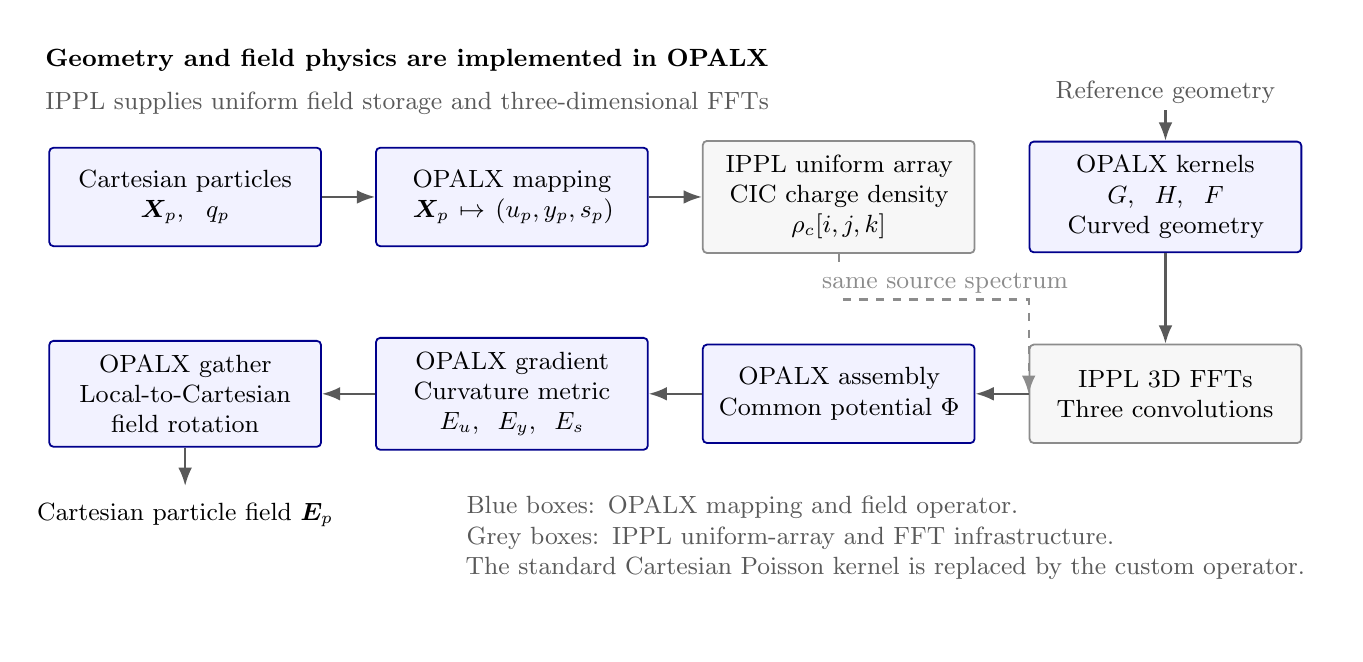
\begin{tikzpicture}[
 x=1cm,y=1cm,font=\small,>=Latex,
 mgop/.style={draw=blue!55!black,fill=blue!5,line width=.65pt,
   rounded corners=1.5pt,align=center,text width=3.1cm,minimum height=1.25cm,inner sep=5pt},
 mgippl/.style={draw=black!45,fill=black!3,line width=.65pt,
   rounded corners=1.5pt,align=center,text width=3.1cm,minimum height=1.25cm,inner sep=5pt},
 mgflow/.style={->,line width=.8pt,black!65},
 mgflowlabel/.style={fill=white,inner sep=2pt,align=center}
]
 \path[use as bounding box] (0,0) rectangle (16.6,7.7);
 \node[anchor=north west,font=\bfseries\small] at (.1,7.55)
   {Geometry and field physics are implemented in OPALX};
 \node[anchor=north west,black!65] at (.1,7.0)
   {IPPL supplies uniform field storage and three-dimensional FFTs};

 \node[mgop] (mga) at (2.0,5.55)
   {Cartesian particles\\$\bm X_p,\;q_p$};
 \node[mgop] (mgb) at (6.15,5.55)
   {OPALX mapping\\$\bm X_p\mapsto(u_p,y_p,s_p)$};
 \node[mgippl] (mgc) at (10.3,5.55)
   {IPPL uniform array\\CIC charge density\\$\rho_c[i,j,k]$};
 \node[mgop] (mgd) at (14.45,5.55)
   {OPALX kernels\\$G,\;H,\;F$\\Curved geometry};
 \draw[mgflow] (mga) -- (mgb);
 \draw[mgflow] (mgb) -- (mgc);
 \draw[mgflow] (14.45,6.65) -- (mgd.north)
   node[pos=0,above,mgflowlabel] {Reference geometry};

 \node[mgippl] (mge) at (14.45,3.05)
   {IPPL 3D FFTs\\Three convolutions};
 \node[mgop] (mgf) at (10.3,3.05)
   {OPALX assembly\\Common potential $\Phi$};
 \node[mgop] (mgg) at (6.15,3.05)
   {OPALX gradient\\Curvature metric\\$E_u,\;E_y,\;E_s$};
 \node[mgop] (mgh) at (2.0,3.05)
   {OPALX gather\\Local-to-Cartesian\\field rotation};
 \draw[mgflow] (mgd) -- (mge);
 \draw[mgflow] (mge) -- (mgf);
 \draw[mgflow] (mgf) -- (mgg);
 \draw[mgflow] (mgg) -- (mgh);

 \node[anchor=north,align=center] at (2.0,1.78)
   {Cartesian particle field $\bm E_p$};
 \draw[mgflow] (mgh.south) -- (2.0,1.88);
 \draw[mgflow,dashed,black!45] (mgc.south) -- ++(0,-.58) -| (mge.west)
   node[pos=.28,above,mgflowlabel] {same source spectrum};
 \node[anchor=west,text width=10.7cm,align=left,black!65] at (5.45,1.22)
   {Blue boxes: OPALX mapping and field operator.\\
    Grey boxes: IPPL uniform-array and FFT infrastructure.\\
    The standard Cartesian Poisson kernel is replaced by the custom operator.};
\end{tikzpicture}

 \caption{Division of responsibility in the implemented OPEN calculation.
 OPALX handles the physical geometry, source interpretation, custom kernels,
 metric gradient and field rotations. IPPL stores ordinary uniform arrays
 and performs FFTs. The existing Cartesian Poisson operator is not used for
 this curved-source convolution.}
 \label{fig:mg-pipeline}
\end{figure}

The source array is transformed once per solve. For each of $G,H,F$, the
backend constructs the cell-integrated kernel, transforms it, multiplies its
spectrum by the same source spectrum, inverse-transforms and accumulates the
appropriate term of \cref{eq:mg-three-convolutions}. FFT plans and work arrays
persist while the mesh shape and spacing remain unchanged. A straight source
needs only $G$; the curved source uses all three kernels.

The discrete FFT is periodic algebraically, so the code embeds the density
in zero-padded arrays to evaluate a free-space linear convolution. In each
direction, the padded length is an even 2/3/5-smooth integer at least $2N+4$.
The extra support accommodates the two-cell potential halo. This numerical
padding does not introduce a physical conducting boundary or a periodic beam.
The singular flat-cell kernel integrals are analytic; a smooth
curved-minus-flat correction is evaluated by quadrature.

For the curved electrostatic case, all local electric components come from
the same potential:
\begin{equation}
 E_u=-\partial_u\Phi^{(1)},\qquad
 E_y=-\partial_y\Phi^{(1)},\qquad
 E_s=-\frac1h\partial_s\Phi^{(1)}.
 \label{eq:mg-field}
\end{equation}
Physical-cell derivatives use fourth-order centred differences. OPALX
interpolates these components to each particle in logical coordinates and
then rotates them into Cartesian directions:
\begin{equation}
 \bm E_{\rm Cartesian}
 =E_u\bm e_u(s)+E_y\bm e_y+E_s\bm e_s(s).
 \label{eq:mg-rotate}
\end{equation}
The geometry used for mapping, field evaluation and rotation is consistent
within one common solve frame. Interpolating without the metric factor, or
returning local components as fixed Cartesian components, would change the
physical result.

\clearpage
\subsection{Computational cost and the change from a slice model}
The conventional slice calculation solves transverse Poisson problems
independently and supplies a separate local longitudinal approximation.
The revised OPEN backend couples the entire deposited three-dimensional
source. It retains the FFT2D5 interface and reference-path organization, but
has genuine three-dimensional FFT cost.

\begin{center}\small
\begin{tabular}{p{0.21\linewidth}p{0.33\linewidth}p{0.36\linewidth}}\toprule
Property & Retained slice/pipe calculation & Revised free-space OPEN\\\midrule
Transverse coupling & Within each transverse slice & Across the finite source\\
Longitudinal field & Separate local closure & Gradient of a common nonlocal potential\\
Numerical transforms & Repeated transverse 2D FFTs & Three-coordinate FFT convolutions\\
Geometry treatment & Local reference-path slices & Smooth circular map and first-order curved-source kernel\\
PyORBIT control & Straight conducting-pipe longitudinal model & Not a curved free-space cross-code comparison\\\bottomrule
\end{tabular}
\end{center}

For $N=N_uN_yN_s$, a three-dimensional transform scales as $O(N\log N)$,
with additional work for the three kernel convolutions. Padding is required
in all three directions. Persistent convolution storage includes one padded
real field, two half-complex fields and an unpadded potential with a halo;
the deposited fields, particle arrays and FFT workspaces add further memory.
Measured peak native-run memory was approximately 13.8 GB for
$64\times32\times8192$ and 27.1 GB for $96\times48\times8192$.
These are whole-run measurements, not the byte count of one grid or a
universal memory forecast.

The reference-path coordinates still save the large empty space inside the
bend. A Cartesian box spanning metre-scale orbit dimensions would require
many cells unrelated to the millimetre-scale beam cross-section if comparable
resolution were imposed. The coordinate-array approach avoids that geometric
cost, but does not retain the computational cost of independent 2D slices.

Nonlocal source coupling is needed to reproduce the finite curved Coulomb
reference being tested. A 3D FFT is one way to evaluate it, not a mathematical
necessity. A reduced approach could combine local transverse solves with a
nonlocal longitudinal/curvature correction or a hierarchical interaction
method. Such an efficient replacement has not been demonstrated here.
Agreement of the present OPEN backend with SACR therefore validates a
different, more expensive operator; it does not prove that the earlier
inexpensive slice approximation meets the same curved-beam target.

\clearpage
\subsection{Validation scope, restrictions and code correspondence}
The completed comparison uses $Q=10$ pC, $\beta=0.001$, the geometry in
\cref{fig:mg-geometry} and uniform or triangular physical longitudinal density.
It tests native particle deposition, solution and gathering against the
independent exact-geometry SACR reference. The primary-grid maximum pointwise
relative errors over the original 43 sampled positions per profile are
\begin{center}\small
\begin{tabular}{lrrr}\toprule
Profile & Radial $E_u$ & Vertical $E_y$ & Tangential $E_s$\\\midrule
Uniform & 0.07084\% & 0.07789\% & 0.55443\%\\
Triangular & 0.06613\% & 0.08660\% & 0.08299\%\\\bottomrule
\end{tabular}
\end{center}
Those positions are at least 5 mm inside the source ends. Across the seven
qualified fine/control cases, the worst nonzero-component relative error is
0.56413\%. The extra uniform-source diagnostic 0.1 mm inside a sharp end
still has 20.66\% tangential error. There is no claim of 1\% accuracy at every
position, or of validated self-consistent tracking.

The current implementation has the following restrictions:
\begin{itemize}
 \item Straight references or horizontal constant-curvature circular arcs
 shorter than one turn, followed by a common rigid solve-frame transformation.
 General paths and closed rings are rejected; near-full-turn accuracy is untested.
 \item One MPI rank and $\max|\kappa u|\le0.01$ across the coordinate domain
 and two-cell potential halo. Every source particle needs a half-cell CIC margin.
 \item Curved fields use instantaneous electrostatics. The code rejects
 $\beta>0.1$, but that cutoff is not a componentwise 1\% error guarantee.
 The local magnetic-field prescription is not a nonlocal Biot--Savart solve;
 retardation, radiation and relativistic curved tracking are unvalidated.
 \item Straight references instead use a common mean-$\gamma$ longitudinal
 stretch and field transformation. The curved formulas above use $\gamma=1$.
\end{itemize}

\begin{center}\small
\begin{tabular}{p{0.43\linewidth}p{0.51\linewidth}}\toprule
Implementation component & Responsibility\\\midrule
\code{FFT2D5Geometry} & Fit supported references; map positions and construct the local basis\\
\code{FFT2D5FieldStorage} & Uniform IPPL coordinate arrays and retained slice workspace\\
\code{FFT2D5Algorithm} & Common solve frame, CIC deposition/gathering, coverage checks and rotations\\
\code{FFT2D5FreeSpaceKernel.h} & Cell-integrated $G,H,F$ kernels and curved chord\\
\code{FFT2D5FreeSpace} & Padded 3D FFT convolutions, potential assembly and metric gradient\\\bottomrule
\end{tabular}
\end{center}
The separate straight conducting-pipe comparison with PyORBIT tests the
retained local model: its maximum OPALX--PyORBIT slice-field difference is
0.447\%. It is not independent cross-code validation of this nonlocal curved
OPEN operator. No simulation or production-code change is introduced by this
explanation.

\end{document}
